\documentclass{standalone}

\usepackage[euler-digits]{eulervm}

\usepackage{tikz}
\tikzset{every node/.style={circle,draw,minimum size=6mm,inner sep=0pt}}
\tikzset{t/.style={rectangle}}

\begin{document}
    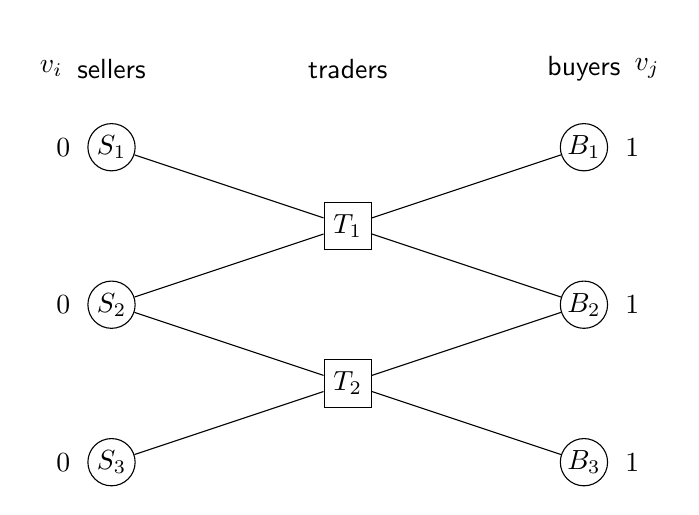
\begin{tikzpicture}[font=\sffamily]
      \node[label=left:{$0$}] (S1) at (-3,4) {$S_1$}; 
      \node[label=left:{$0$}] (S2) at (-3,2) {$S_2$}; 
      \node[label=left:{$0$}] (S3) at (-3,0) {$S_3$}; 
      \node[label=right:{$1$}] (B1) at (3,4) {$B_1$}; 
      \node[label=right:{$1$}] (B2) at (3,2) {$B_2$}; 
      \node[label=right:{$1$}] (B3) at (3,0) {$B_3$}; 
      \node[t] (T1) at (0,3) {$T_1$}; 
      \node[t] (T2) at (0,1) {$T_2$}; 
      \foreach \a/\b in {S1/T1,S2/T1,S2/T2,S3/T2}
        \draw (\a) -- (\b);
      \foreach \a/\b in {B1/T1,B2/T1,B2/T2,B3/T2}
        \draw (\a) -- (\b);
        \node[label=left:{$v_i$},draw=none] (S) at (-3,5) {sellers};
        \node[label=right:{$v_j$},draw=none] (B) at (3,5) {buyers};
        \node[draw=none] (T) at (0,5) {traders};
    \end{tikzpicture}
\end{document}
